\documentclass[twoside,english]{uiofysmaster}
\usepackage[utf8]{inputenc}
\usepackage[T1]{fontenc}
\usepackage[english]{babel}
\usepackage{epsfig}
\usepackage{graphicx}
\usepackage{caption}
\usepackage{subcaption}
\usepackage{amsfonts, amssymb, amsmath}
\usepackage{listings}
\usepackage{float}
\usepackage[top=2cm, bottom=2cm, left=2cm, right=2cm]{geometry}
\usepackage{hyperref}
\usepackage{epstopdf}


\usepackage[]{biblatex}
% \bibliography{bibtex_ref_test.bib}
\bibliography{references.bib}

\renewcommand{\d}{\partial}

\setlength{\headheight}{15pt}

% \usepackage{fontspec}
% \newfontfamily\listingsfont[Scale=0.85]{Droid Sans Mono}
% \lstset {
%     basicstyle=\footnotesize\listingsfont,
%     keywordstyle=\color{listingskeywordcolor}\footnotesize\listingsfont,
%     stringstyle=\color{listingsstringcolor}\footnotesize\listingsfont,
%     commentstyle=\color{listingscommentcolor}\footnotesize\listingsfont,
%     numberstyle=\color{listingsnumbercolor}\footnotesize\listingsfont,
%     identifierstyle=\footnotesize\listingsfont,
% }



% compile with pdflatex --shell-escape main.tex


%opening
\author{Fredrik E Pettersen\\ f.e.pettersen@fys.uio.no}
\title{\uppercase{Multiscale modeling of diffusion processes in the brain}}
\date{June 2013}
\begin{document}


\maketitle

\begin{abstract}
This is an abstract text.
\end{abstract}

% \begin{dedication}
%   To someone
%   \\\vspace{12pt}
%   This is a dedication to my cat.
% \end{dedication}

\begin{acknowledgements}
  I acknowledge my acknowledgements.
\end{acknowledgements}


\tableofcontents
\clearpage
\listoffigures
\clearpage
\listoftables

\chapter{Introduction}
This thesis is an attempt at modeling diffusion processes in which part of the process takes place on a length scale so small that the continuum approximation becomes invalid. 
In this part we will therefore try and introduce another model of the diffusion process in the hope that this will give us something extra. 
It is the hope of Hans Petter that this thesis will be an introduction to a new research project to understand mesoscale physics in collaboration with Gaute Einevoll at UMB.

The very first approach was to simply try the problem on a bit. That is to try and substitute some small part of the mesh in a Finite Difference Diffusion solver (Froward Euler scheme) with a stochastic diffusion solver. A random walk method was implemented on part of the mesh to take over the equation-solving. This was done in 1 and 2 spatial dimensions with the aim of finding potential difficulties so that we can further investigate them. \\
Upon switching length-scales a fundamental question arises almost immediately; what is the continuum limit? In our case this question takes a slightly different, and possibly more answerable form; what is the conversion rate between the continuum model and the microscopic model, and by extension, what does a walker correspond to?
The first instinct of this candidate was to just try some conversion rate (say some value corresponds to some number of walkers), and this was implemented in both 1 and 2 dimensions.

\section{Background}
\emph{This is very much a first draft, and only my thoughts around what I understand as the basis of the thesis.}\\
Though the scope of this thesis might seem a bit \emph{sought}, it is in fact a real world concern from the computational neuroscience group at UMB. 
Their work contains network simulations of neurons, which they are trying to tweak with experimental data. 
The experimental data come from measurements of voltage levels in the Extra Cellular Space (ECS). 
The ECS is, essentially, the space which separates neurons and has an immensely complicated geometry as we can see from figure \ref{ECS_picture}. 
The width of the ECS varies, but is in general $\sim1\mu$m. 
Parts of the ECS is, however, much narrower. In the ECS there are a number of diffusion governed transport mechanisms which are vital for the function of the neurons. 
In fact, there are examples of snake venom which have a shrinking effect on the ECS, and it is thought that this causes large scale neuronal death very quickly. 
For the researchers at UMB, however, the ECS is of importance because the diffusion tensor in the ECS is related to the conductivity tensor through equation \ref{conductivity_diffusion_eq}, which in turn lets them teak parameters in their network models. \\
\begin{equation}\label{einstein_viscosity}
D = \frac{k_B T}{6\pi \eta r},
\end{equation}
Though there are several reasons to study diffusion processes in the ECS, this project has a specific goal in mind. 
The Einstein relation, eq. (\ref{einstein_viscosity}), relates the diffusion constant to the viscosity of the medium in which the diffusion is taking place. 
From the definition of viscosity, $\mu$, we have 
\begin{equation}
v_d = \mu F 
\end{equation}
where $F = qE$ is the standard electrical force acting on a charged particle. 
We can also define the current from the drift velocity of the particles as 
\begin{equation}
J = cqv_d = \sigma E 
\end{equation}
where $\sigma = c\mu q^2$ is the electrical conductance, in this case, of the ECS. 
Inserting this in the Einstein relation, eq. (\ref{einstein_viscosity}), lets us express the conductivity in terms of the diffusion constant as 
\begin{equation}\label{conductivity_diffusion_eq}
\sigma = \frac{cq}{k_B T}D 
\end{equation}
Equation (\ref{conductivity_diffusion_eq}) is trivially generalizable to tensor notation, where the conductance and diffusion ``constant'' are both 2. order tensors.\\

\begin{equation}\label{stochastic_einstein}
\langle r^2\rangle = 2dDt 
\end{equation}

The fundamental problem here is that, while diffusion in its own is a truly multi-scale process, we have no way of knowing for sure that the continuum models, and all they bring with them, are correct for this type of geometry. 
In particular, the Einstein relation \ref{einstein_viscosity} has, to my knowledge, only been derived for diffusion in a homogeneous media. 
The definition of a homogeneous media includes a mean free path close to infinity, which we will have trouble arguing for the existence of in the ECS. 
On the other hand, I know that another Einstein relation \ref{stochastic_einstein} is widely used  in other fields of physics where the media in question is hardly homogeneous. 
In molecular dynamics simulations, the two mentioned Einstein relations are used to measure the viscosity of fluids in nano-porous materials, and with success as far as I know.

\section{A short introduction to mathematical neuroscience}

Neuroscience is the scientific study of the nervous system, but in the traditional sense it focuses very much on what parts of the brain are responsible for what. 
Mathematical neruroscience is more focused on the physics and chemistry involved in the different parts of the brain and nervous system. 
An example of the power of this approach is the classical work done by Hodgkin and Huxley in 1952, earning them the Nobel price in Physiology or medicine in 1963. 
Through four non-linear coupled differential equations they were able to predict the propagation speed of signals along the squid giant axon to a quite high precision. \\

% Copied from the project

The human brain consists of two types of cells; the neurons and neuroglia. 
Neurons are tasked with signal processing and transport, while the glia are thought to have more janitorial tasks. 
The neurons are bathed in a salt solution that is mainly $Na^+$ and $Cl^-$. 
Inside the neurons, a highly regulated salt solution of mainly $K^+$ sets up a potential difference relative to the outside of the cell of approximately $-65$mV.
The neurons are in constant communication with each other through action potentials, which are disturbances in the membrane potentials of neurons. 
These action potentials are generated in the body of the cell, called the soma, from where they propagate down the axon without loss of amplitude. 
This is achieved by constantly amplifying the signal using ion pumps (see the Hodgin-Huxley model of the action potential \cite{graham2011principles}).
After propagating down the axon, the action potential reaches a synapse which is a gate to another neuron. 
If the action potential is of significant strength, vesicles carrying neurotransmitters merge with the synapse membrane, letting the neurotransmitters diffuse to the dendrite of the other neuron. 
If enough neurotransmitters reach the post-synaptic side, the signal continues propagating to the soma of this neuron, and the entire process starts over again. \\
The interest of this project lies, mainly, in the diffusion processes that take place in the space between these types of cells, the so-called extracellular space (ECS). 
This is a narrow space ($\sim 10-100$ nm \cite{nicholson2001diffusion}) with a highly complicated geometry (Figure \ref{ECS}). 
Surprisingly, the ECS adds up to $20\%$ of the total brain volume. 
We can understand this by realizing that every part of a cell must be separated from another cell by the ECS. 
Since the cells consists of axons and dendrites which can be viewed as (somewhat) fractal, we see that this means separating a vast amount of surface area from other surface areas.

The ECS is thought to support the diffusion of oxygen and nutrients to the neurons and glia, and diffusion of carbon dioxide and other waste from these cells through the blood - brain barrier and into the bloodflow. 

% \section{Dendritic spines}




\chapter{Basic Theory}
In this chapter we will take a closer look at random walks, both in general and the transition from the statistical view to partial differential equations. 
We will take a look at different algorithms to produce random walks, and discuss their pros and cons in light of this project.

\section{Introduction to random walks}
The most basic random walk is a walker on the x-axis which will take a step of a fixed length to the right with a probability $p$, or to the left with a probability $q=1-p$. 
Using (pseudo-) random numbers on a computer we can simulate the outturn of a random walk. 
For each step (of which there are N) we draw a random number, r, between 0 and 1 from some distribution (say a uniform one) which will be the probability. 
If $r\leq p$ the walker will take a step to the left, otherwise it will take a step to the left. 
After the N steps the walker will have taken R steps to the right, and $L = N-R$ steps to the left. 
The net displacement from the origin will be $S = R-L$. 

\subsection{Further discussion and analysis of the introduction}
If we do sufficiently many walks, the net displacement will vary from $S=+N$ to $S=-N$ representing all steps to the right and all steps to the left respectively. 
The probability of all steps beeing to the right is $P_N(N) = p^N$. 
Should one of the steps be to the left, and the rest to the right we will get a net displacement of $S = N-2$ with the probability $P_N(R = N-1) = Np^{N-1}q$. 
We can generalize this to finding the probability of a walk with a R steps to the right as 
\begin{equation}\label{bernoulli_distr}
 P_N(R) = {N\choose R}p^{R}q^{N-R}
\end{equation}
where ${N\choose R}=\frac{N!}{R!(N-R)!}$ is the number of walks which satisfy the net displacement in question, or the multiplicity of this walk in statistical mechanics terms. 
Equation \ref{bernoulli_distr} is the Bernoulli probability distribution, which is normalized.
\begin{align*}
 \sum\limits_{R=0}^N P_N(R) = (p+q)^N = 1^N = 1
\end{align*}
We can use this distribution to calculate various average properties of a walk consisting of N steps. 
For example, the average number of steps to the right is
\begin{align*}
 \langle R\rangle &=  \sum\limits_{R=0}^N RP_N(R) =  \sum\limits_{R=0}^N {N\choose R}Rp^Rq^{N-R} = \\
 p\frac{d}{dp} \sum\limits_{R=0}^N {N\choose R}p^Rq^{N-R} &= p\frac{d}{dp}(p+q)^N = Np(p+q)^{N-1} = Np
\end{align*}
From this we can also find the average value of the net displacement using $S = R-L = R-(N-R) = 2R-N$.
\begin{align*}
 \langle S\rangle = \langle2R\rangle -N = 2Np-N\underbrace{(p+q)}_{=1} = N(2p-p-q) = N(p-q)
\end{align*}
We notice that the average net displacement is greatly dependent on the probability of the walk and that any symmetric walk will have an expected net displacement of zero. 
In many cases we will be more interrested in the mean square displacement than the displacement itself. 
This can also be calculated rather straightforwardly. 
\begin{align*}
  \langle R^2\rangle =  \sum\limits_{R=0}^N R^2P_N(R) &=  \sum\limits_{R=0}^N {N\choose R}R^2p^Rq^{N-R} = \\
 \left(p\frac{d}{dp}\right)^2 \sum\limits_{R=0}^N {N\choose R}p^Rq^{N-R} &= \left(p\frac{d}{dp}\right)^2(p+q)^N \\
 = Np(p+q)^{N-1} +p^2N(N-1)(p+q)^{N-2} &= (Np)^2 +Np(1-p) = (Np)^2 +Npq
\end{align*}
Like before, the average nett displacement is given as $S^2 = (2R-N)^2$ and we obtain
\begin{align*}
 \langle S^2\rangle = 4\langle R^2\langle -4N\langle R\rangle + N^2 &= 4((Np)^2 +Npq) -4N^2p + N^2\\
 = N^2(4p^2 -4p +1) +4Npq &= N^2(2p-1)^2 +4Npq = N^2(p-q)^2 +4Npq
\end{align*}
which for the 1D symmetric walk gives $\langle S^2\rangle =N$




\chapter{Analysis}
\section{Some discussion}

This chapter will concern most of the numerical error analysis and som of the discussion of this analysis as well as an introduction to the methods used for error analysis in general, and how they are adapted to this particular problem.\\


In this numerical setup we will potentially introduce several new error sources in addition to the nomal errors introduced by numerical solution of any equation (see section \ref{some_words_on_PDEs}). 
When a part of the solution acquired is replaced by the solution from another model, which in this case is stochastic, we will change the initial condition to the next iteration in time. 
This might have a number of effects on our final solution. 
When we solve a differential equation numerically we only get an approximation to the actual solution because we are using approximate derivatives (see figure \ref{illustrate_approximate_derivatives}). 
To investigate the error we are introducing we will first need to test that the truncation error of the numerical PDE solver behaves as expected. 
% This can be done by chosing a solution to the PDE, doing a simulation which should yield the same solution and then comparing the two answers. 
% As argued in section \ref{} we will struggle with making the error from the random walk solver be much smaller than $\mathcal{O}(\Delta t)$. 
% We will therefore start by using a simple discretization of the PDE which also has a truncation error of $\mathcal{O}(\Delta t)$. 
% Figure \ref{errorplot_1d} shows the error norm (\ref{}) of only the PDE solver done in 1 dimension plotted for each timestep of the simulation. 
% The manifactured, exact solution is $u(x,t) = \exp\left(-\pi^2t\right)\cos(\pi x)$ and its initial condition is shown in figure \ref{}.

\begin{figure}[H]
 \centering
 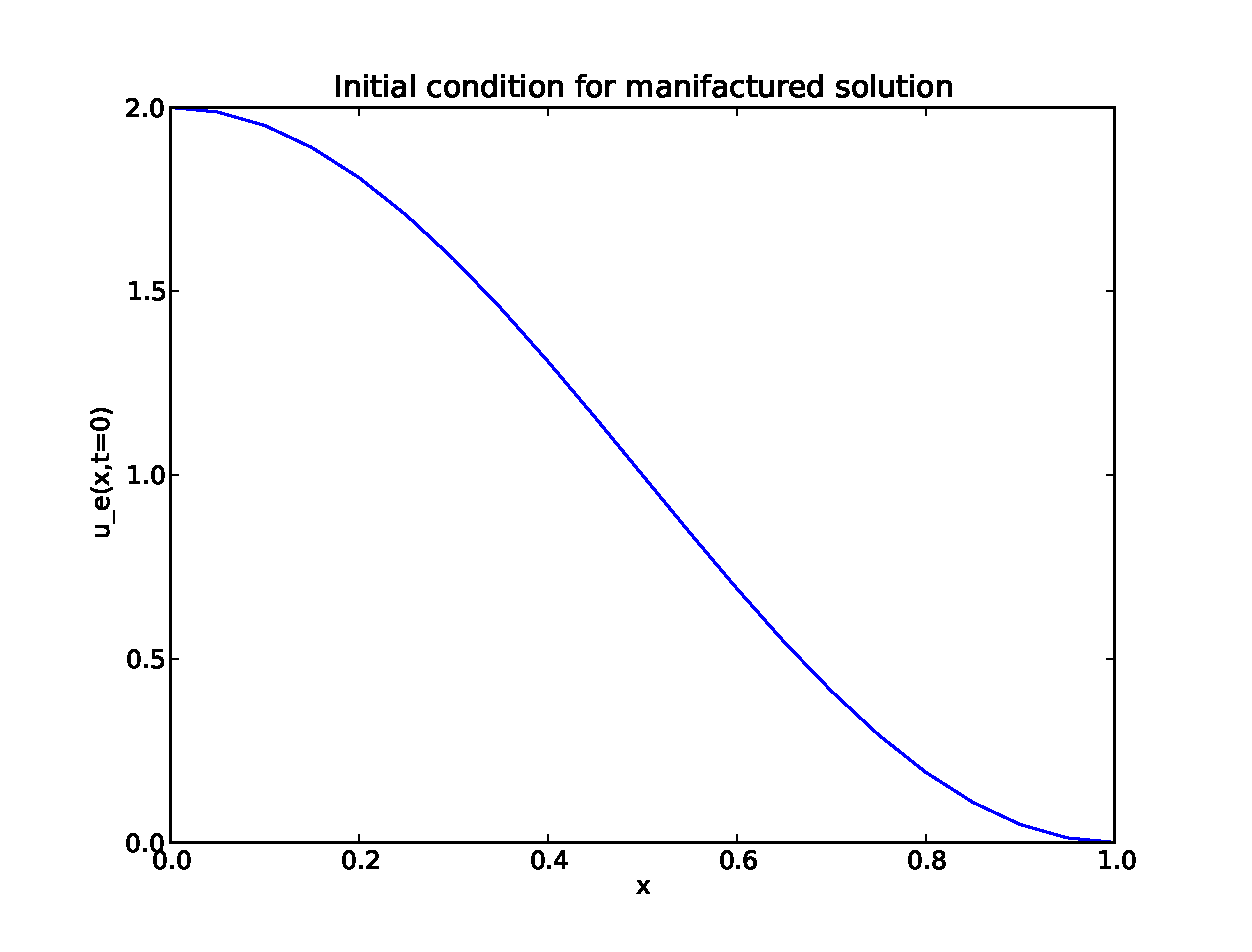
\includegraphics[scale=0.7]{/home/fredriep/Dropbox/uio/thesis/doc/results/experiment_31102013_1017/results/initial_condition.eps}
 \caption[Initial condition in 1d]{Initial condition of manifactured solution in 1d and the simulation.}
 \label{initial_condition_1d}
\end{figure}


\section{Manifactured Solutions}
A normal way of checking that our scheme of choise is implemented correctly is by making an exact solution to the equation and checking that the error is of the expected order. 
As a first, simple implenetation we have worked with the explicit Forward Euler discretization of the simplest form of the diffusion equation \ref{simple_diffusion_equation}. 
This discretization is expected to have an error-term of the order of $\Delta t$, which again is limited by a stability criterion. 
We can now decide that the solution to equation \ref{simple_diffusion_equation} should be
\begin{equation}\label{manifactured_solution_1D}
 u(x,t) = e^{-t\pi^2}\cos(\pi x) +1
\end{equation}
which satisfies our equation if we set the diffusion constant to 1.
\begin{align}
 \frac{\d }{\d t}e^{-t\pi^2}\cos(\pi x) +1 &= D\frac{\d^2}{\d x^2}e^{-t\pi^2}\cos(\pi x) +1\\
 -\pi^2e^{-t\pi^2}\cos(\pi x) &= -\pi^2e^{-t\pi^2}\cos(\pi x) +1 \implies 1 = 1
\end{align}
As we saw in section \ref{truncation_error} the Forward Euler scheme is expected to have an error of the order of $\Delta t$. 
Testing only the scheme first, in 1D we get the following plot \ref{errorplot_FE1D_noWalk} of the maximum of the absolute value of the difference between the exact solution and the numerical solution to the equation. 

\begin{figure}[H]
\centering
\includegraphics[scale=0.7]{/home/fredriep/Dropbox/uio/thesis/doc/results/experiment_31102013_1017/results/deterministic_errorplot.eps}
\caption[Numerical error for 1D Forwar Euler discretization]{Numerical error for 1D Forwar Euler discretization of the PDE. Nothing else is done to the simulation.}
\label{errorplot_FE1D_noWalk}
\end{figure}

We then introduce an area on the domain where we swich models from the normal PDE to an average of the PDE solution and the result of a random walk simulation where the initial condition is the last timestep from the PDE converted to walkers by the conversion rate given in equation \ref{conversion_rate}. In this case we have used the parameters $a=3$, $\Delta t = \frac{\Delta x^2}{3.0}$, $\Delta x = \frac{1}{20}$. 
These parameters makes one unit of $u(x,t)$ equal to some $1000$ walkers. 
\begin{equation}\label{conversion_rate}
 C_{ij} = \frac{a}{\Delta t}U_{ij}
\end{equation}
The area where the model has been replaced is between $x=0.6$ and $x=0.7$, which is three mesh points. 
In the same way as for only the simple 1D PDE case we compare the combined numerical solution from the two models to the exact solution. 
Figure \ref{errorplot_FE1D_Walk_first_attemt} shows that the error is still of the order of $\Delta t$, and the difference between the two models are negligable. 

\begin{figure}[H]
\centering
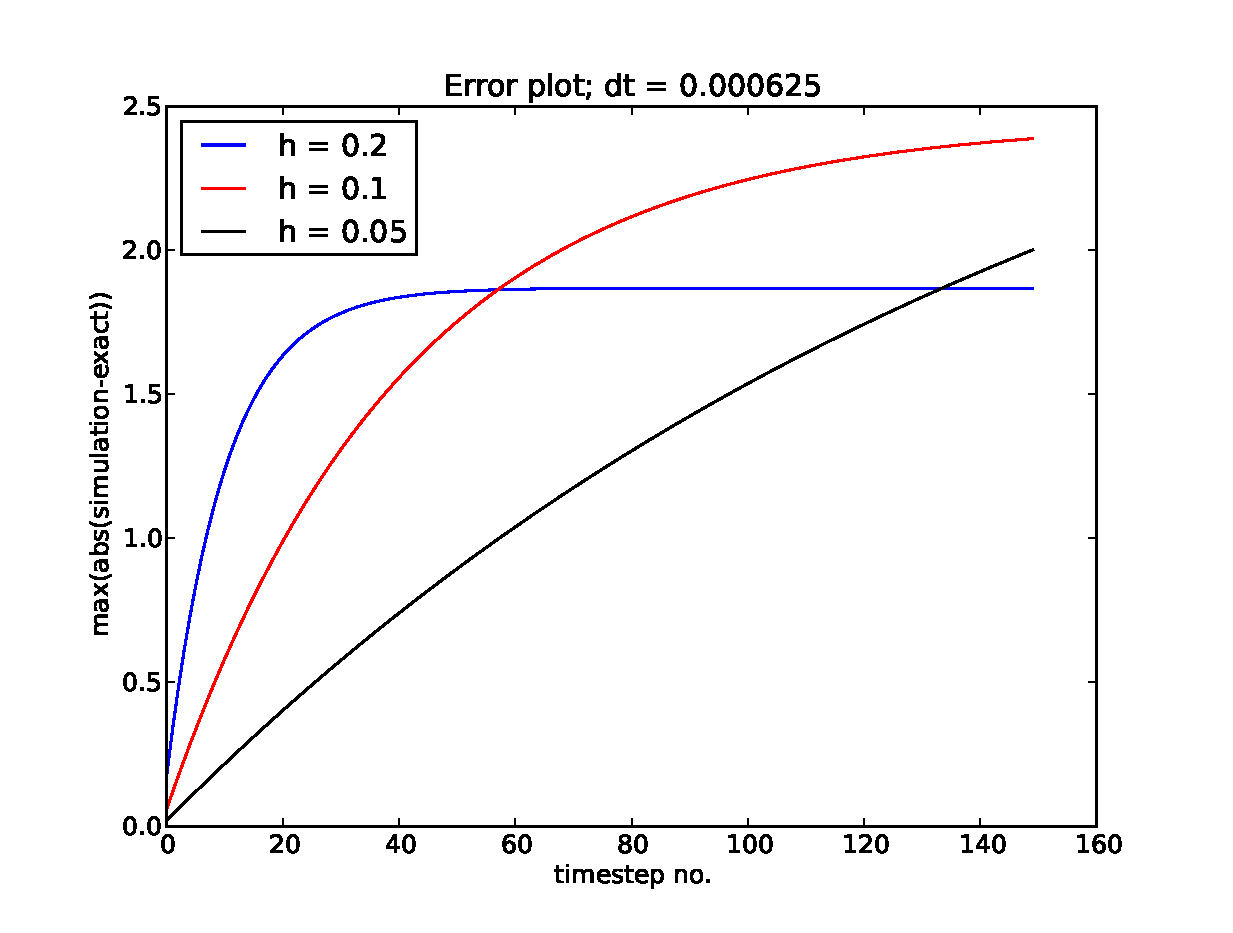
\includegraphics[scale=0.7]{/home/fredriep/Dropbox/uio/thesis/doc/results/experiment_31102013_1017/results/errorplot.eps}
\caption[Effect of increasing number of walkers]{Numerical error for 1D Forward Euler discretization combined with random walk model between $x=0.6$ and $x=0.7$. Other parameters of importance are $\Delta t\approx 0.00083333$, $\Delta x = 0.05$.}
\label{errorplot_FE1D_Walk_first_attemt}
\end{figure}

As we can se from figure \ref{errorplot_FE1D_Walk_first_attemt} increasing the number of walkers that each ``unit concentration'' corresponds to has a positive effect on the errornorm up to a certain point. 
After we reach $Hc \sim 10^4$ the error is dominated by the truncation error of the Forward Euler scheme. 
This tells us that the error associated with introducing a random walk model on parts of the mesh behaves roughly as we hoped; it tends to zero for large numbers of walkers. 
Meaning of course that the calculations in section \ref{} are not hopeless.



\subsection{The effects of adding drift to the walkers}

As shown in section \ref{random_walks_and_drift} adding drift to the walkers will modify our model to represent the convection diffusion equation (\ref{convection_diffusion_equation}) rather than the simple diffusion equation. 
In our analysis so far we have completely ignored the spatial truncation error because it is of second order, and the truncation error in time is of first order. 
When discretizing the convection diffusion equation however, we must take care to use an approximation to the first order spatial derivative that has a truncation error of second order. 
Otherwise the truncation error in this term will completely dominate seeing as $\Delta t<\Delta x$. 
We must also find a new stability criterion for the scheme. \\
As for now, the Leap-frog discretization will do (though it is not by far a perfect choise seeing as it is unstable). 
As a sidenote we can also note that the Neumann boundary condition will be very clear in this scheme. 
$\frac{\d C}{\d n} = 0 \implies \frac{\d C}{\d x} = 0 $ on the boundary, leading to $C_{-1} = C_{1}$ on the boundary and cancelling the drift term on the boundary.
\begin{equation}\label{convection_diffusion_equation_leapfrog}
 C^{n+1} = \frac{D\Delta t}{\Delta x^2}\left(C^n_{i+1}-2C^n_i+C^n_{i-1}\right)-\frac{v\Delta t}{2\Delta x}\left(C^n_{i+1}-C^n_{i-1}\right) + C^n
\end{equation}
The truncation error for the first order derivative using the Leap-frog scheme is obtained as follows
\begin{align*}
 u(t,x+\Delta x) = u(t,x) + \frac{\d u(t,x)}{\d x}\Delta x + \frac{\d^2u(t,x)}{2\d x^2}\Delta x^2 +\mathcal{O}(\Delta x^3)\\
 u(t,x-\Delta x) = u(t,x) - \frac{\d u(t,x)}{\d x}\Delta x + \frac{\d^2u(t,x)}{2\d x^2}\Delta x^2 +\mathcal{O}(\Delta x^3)
\end{align*}
which we recognize as the same error we got from the second order spatial derivatives.\\
If we now do the same analysis as we have already done, by finding a manifactured solution to the convection diffusion equation, implementing a numerical scheme like \ref{convection_diffusion_equation_leapfrog} to solve it after and taking the errornorm. \\
The errornorm does not have to go as $\Delta t$, but it must be halved (approximately) if we halv $\Delta t$. 
Figure \ref{} shows two simulations of equation \ref{convection_diffusion_equation} for $D =1$ and $v=1$ compared to the manifactured solution \ref{manifactured_solution_1D} without adding walkers. 
Before the simulation we must find a source term so the manifactured solution will solve the equation.
\begin{align*}
 -\pi^2\exp\left(-\pi^2t\right)\cos\left(\pi x\right) &= -\pi^2D\exp\left(-\pi^2t\right)\cos\left(\pi x\right) + \pi v \exp\left(-\pi^2t\right)\sin\left(\pi x\right) + f(x,t)\\
 -\pi^2\cos\left(\pi x\right) &= \pi^2D\cos\left(\pi x\right) +\pi v \sin\left(\pi x\right) + \tilde{f}(x) \\
 \tilde{f}(x) &= -\pi\sin\left(\pi x\right)
\end{align*}
Where $f(x,t) = \exp\left(-\pi^2t\right)\tilde{f}(x)$.

\begin{figure}[H]
\centering
\begin{subfigure}[b]{0.48\textwidth}
\includegraphics[width=\textwidth]{/home/fredriep/Dropbox/uio/thesis/doc/results/experiment_05112013_0923/results/deterministic_errorplot.eps}
\caption{}
\label{Verification_convection_diffusion:single_dt}
\end{subfigure}
\begin{subfigure}[b]{0.48\textwidth}
\includegraphics[width=\textwidth]{/home/fredriep/Dropbox/uio/thesis/doc/results/experiment_05112013_0925/results/deterministic_errorplot.eps}
\caption{}
\label{Verification_convection_diffusion:double_dt}
\end{subfigure}
\caption[Verification of Convection diffusion equation implenetation]{Verification of Convection diffusion equation implenetation}
\label{Verification_convection_diffusion}
\end{figure}
As we see from figure \ref{Verification_convection_diffusion} the errornorm is halved when $\Delta t$ is halved, just as we expected. 
We can then advance to testing the effect of adding an area of walkers for different values of $Hc$ as before. 
Note that we have now added some drift to the walkers so the model will fit better.

\section{2D}
Doing the same tests is 2D gives slightly different results; adding a 2D walk-domain has an influence on the error, but a rather small one. 
This can, however be tweaked by increasing the conversion parameters.

\chapter{Results}
\printbibliography
\end{document}

